%!TEX root=writeup.tex
\section{Approach Overview}

\begin{figure}[t]
 \centering
 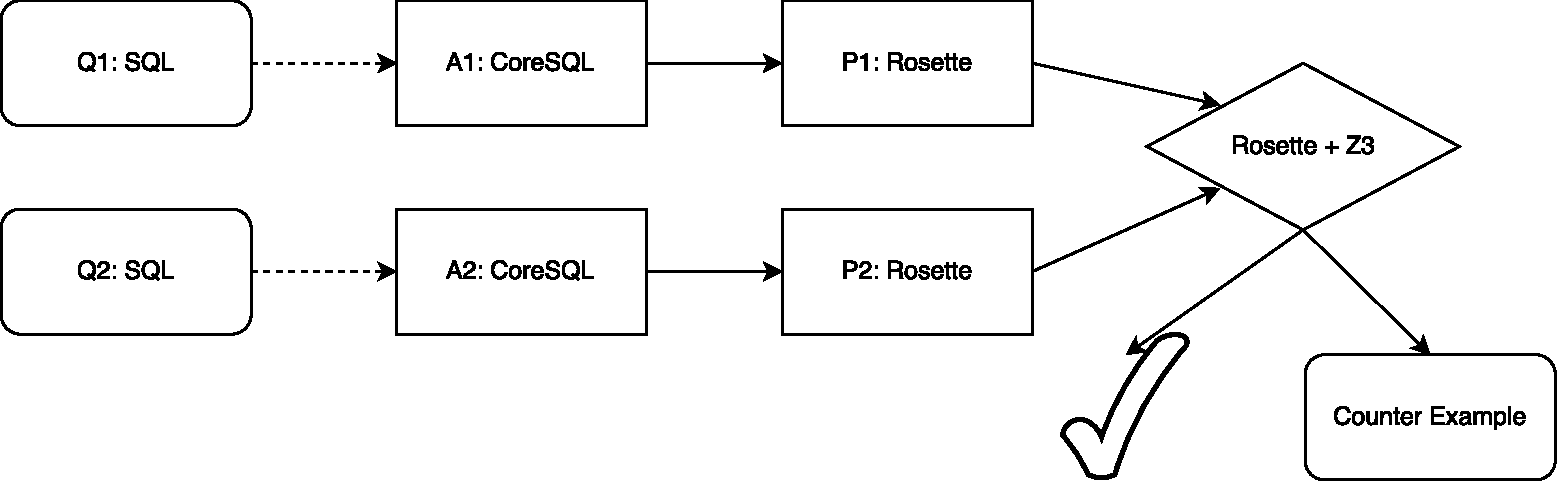
\includegraphics[width=0.7\linewidth]{SymSQLArch}
 \caption{Architecture of Our System}
 \label{fig:arch}
\end{figure}

The Figure~\ref{fig:arch} shows the architecture of our verfication sytem. We define a SQL like DSL $\mathsf{CoreSQL}$ 
(See Section 3 for greater detail) in Racket
to let user write rewriting rules. 
A rewriting rule will be expressed in two $\mathsf{CoreSQL}$ queries.
Our system will denote $\mathsf{CoreSQL}$ queries into Rosette 
\cite{rosette} (See Section 4 for the details of denotation). 
We define our bag semantic equality predicate in Rosette and use it 
to check whether two $\mathsf{CoreSQL}$ queries are equal over 
symbolic tables as input tables. The verifier (the Rosette program) 
will either verify the rewriting rule or output a counter example,
which is a instance of input tables that these two queries will 
have different results.



%%% Local Variables:
%%% mode: latex
%%% TeX-master: "writeup"
%%% End:
